\section{SWE-agent Design}
\label{appx:interface}

\begin{wrapfigure}{r}{0.4\textwidth}
\vspace{-1em}
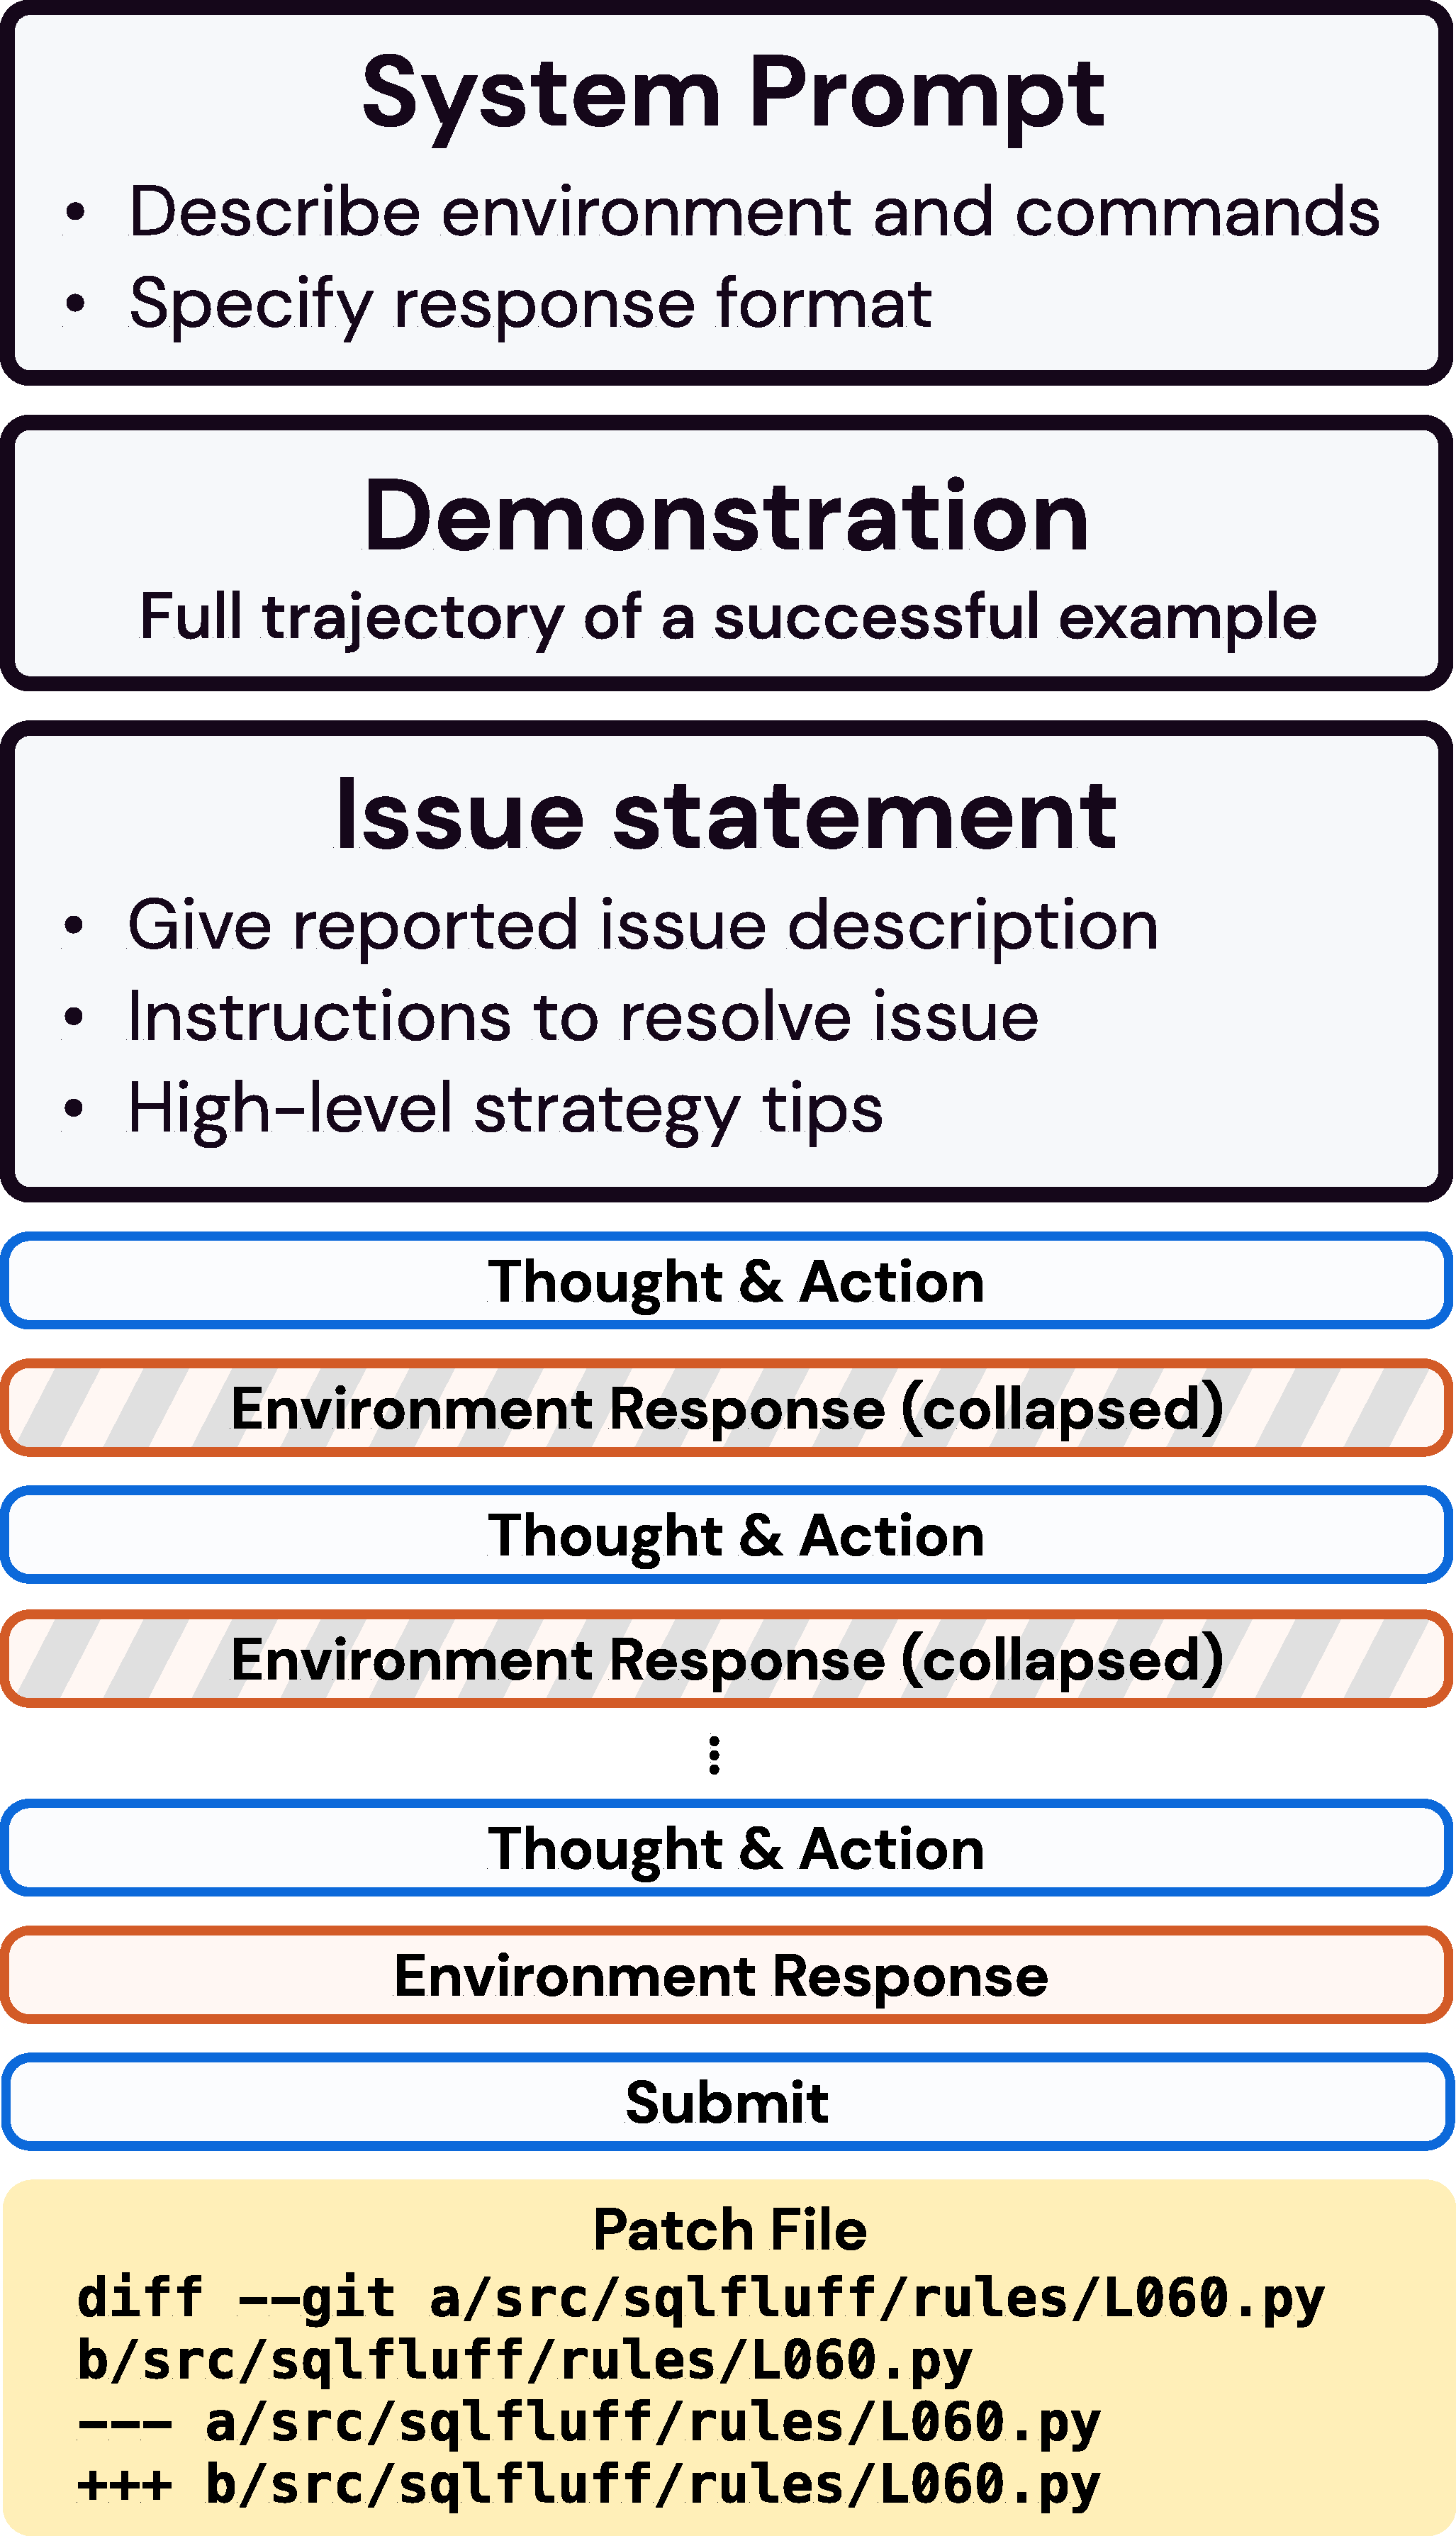
\includegraphics[width=1.0\linewidth]{figures/trajectory_overview.pdf}
    \caption{
    An overview over the structure of a trajectory: We first present the system prompt, demonstration (optional), and issue statement.
    The agent then interacts in turn with the environment. Past observations may be \textit{collapsed}, i.e. we truncate any long output, as described in Section~\ref{sec:sweagent}.
    }
    \label{fig.trajectory_overview}
\vspace{-4em}
\end{wrapfigure}

In this section, we go into greater discussion about the design methodology, appearance, and implementation of each of the SWE-agent components.
As described in Section~\ref{sec:sweagent}, the SWE-agent interface consists of several components that enable agents to accomplish key sub-tasks that are fundamental to solving software engineering problems.
These are generally the following:

\begin{enumerate}[noitemsep,leftmargin=*]
    \item \textit{Localization}: Identify file(s)/line(s) causing the issue.
    \item \textit{Editing}: Generate fixes addressing the given issue.
    \item \textit{Testing}: Write new scripts or modify existing test files to reproduce the issue and/or verify if fixes are correct.
\end{enumerate}

To enable LM-based agents to efficiently carry out these individual functions and progress towards the overarching goal of resolving a codebase issue, we provide a file viewer, file editor, search / navigation system, and context management system.
In Section~\ref{appx:interface:component-design}, we provide a thorough breakdown of each of these components.
In Section~\ref{appx:interface:implementation}, we discuss the technical design decisions and challenges of building SWE-agent.
In Section~\ref{appx:interface:configuration}, we discuss how SWE-agent is configured to support the final interface, along with how SWE-agent is built to enable easy extensibility and customization to alter the interface.

\subsection{ACI Design}
\label{appx:interface:component-design}
In this section, we revisit each component discussed in Section~\ref{sec:sweagent}.
Per section, we first briefly review the component.
We then discuss the underlying motivation for the component with respect to existing software tools.
Finally, we note any additional thoughts that influenced the design process of the component with some occasional discussion of what aspects of the component heavily influence language model behavior.

For a quick, text-free overview, comprehensive documentation for all commands, their usage, and docstrings are included in Table~\ref{tab:commands}.
Figure~\ref{fig.trajectory_overview} visualizes the message history for SWE-agent.
Each prompt template is discussed thoroughly in Section~\ref{appx:prompts}.

\paragraph{File viewer.}
As discussed in Section~\ref{sec:sweagent}, the File Viewer is fundamental to a language agent's ability to understand file content and understand how different programmatic entities relate to one another.
The File Viewer refers to an interface that consists of the four commands, as shown in Table~\ref{tab:commands}, and a customized standard output for displaying \texttt{n} lines of a file at a time.
Using the file viewer, an agent can look at \texttt{n} lines of a file at a time and jump around the file.
The File Viewer enables agents to perform fine-grained localization steps and also understand relationships between intra-file entities.

First, we discuss why existing software systems and graphical user interfaces are sub-optimal for LM use.
In a Shell-only setting, there are several commands that can be used to inspect file content. However, out of the box command line tools are sub-optimal or limiting for language agents for several reasons.
First, commands that print files to standard output (e.g. \texttt{cat}, \texttt{printf}) can easily flood a language agent's context window with too much file content, the majority of which is usually irrelevant to the issue.
Enabling a language agent to filter out distractions and focus on relevant code snippets is crucial to generating effective edits.
While commands like \texttt{head} and \texttt{tail} reduce length to the first/last \texttt{n} lines, it is not intuitive to use bash commands to perform in-file navigation.
It is either impossible or requires a long list of arguments to show specific file lines.
Furthermore, since such Bash commands are stateless, ``scrolling" up/down relative to the current file position typically requires regenerating the same lengthy command with minor changes.
Interactive tools like \texttt{more} and \texttt{less} accommodate this, but (1) representing navigation actions (multiple key up/down clicks) is intuitive for humans, but is verbose and costly for language agents, and (2) even if jumping to a specific line number is allowed, it is not possible to quickly identify what classes/methods/symbols are declared in a file and then immediately go to their definitions.

\begin{table}[t]
\caption{
In additional to the standard Linux Bash commands, we provide SWE-agent with specialized tools, including an interactive file viewer, search functionalities, and edit tools for the open file. Required arguments are enclosed in \texttt{<>} and optional arguments are in \texttt{[]}. The last column shows the documentation presented to the LM.
}
\label{tab:commands}
\vspace{0.25em}
\centering
\begin{tabular}{p{0.08\linewidth}>{\raggedright\arraybackslash}p{0.33\linewidth}p{0.48\linewidth}}
\toprule
\multicolumn{1}{l}{Category}& \multicolumn{1}{c}{Command} & \multicolumn{1}{c}{Documentation} \\
\midrule
% \multicolumn{2}{l}{\textit{File viewer}} \\
% \cmidrule(lr){1-2}
\textit{File viewer} & \textbf{open}\texttt{ <path> [<line\_number>]} & Opens the file at the given path in the editor. If \texttt{line\_number} is provided, the window will move to include that line. \\
\addlinespace
& \textbf{goto}\texttt{ <line\_number>} & Moves the window to show line\_number. \\
\addlinespace
& \textbf{scroll\_down} & Moves the window up 100 lines. \\
\addlinespace
& \textbf{scroll\_up} & Moves the window down 100 lines. \\
% \cmidrule(lr){1-2}
% \multicolumn{2}{l}{\textit{Search tools}} \\
% \cmidrule(lr){1-2}
\cmidrule(lr){1-3}
\textit{Search tools} & \textbf{search\_file}\texttt{ <search\_term> [<file>]} & Searches for \texttt{search\_term} in file. If file is not provided, searches in the current open file. \\
\addlinespace
& \textbf{search\_dir}\texttt{ <search\_term> [<dir>]} & Searches for \texttt{search\_term} in all files in dir. If dir is not provided, searches in the current directory. \\
\addlinespace
& \textbf{find\_file}\texttt{ <file\_name> [<dir>]} & Finds all files with the given name in dir. If dir is not provided, searches in the current directory. \\
% \cmidrule(lr){1-2}
% \multicolumn{2}{l}{\textit{Editing}} \\
% \cmidrule(lr){1-2}
\cmidrule(lr){1-3}
\textit{File \mbox{editing}} & {\textbf{edit} \texttt{<n>:<m>}  \texttt{<replacement\_text>} \textbf{end\_of\_edit}} & Replaces lines n through m (inclusive) with the given text in the open file. All of the \texttt{replacement\_text} will be entered, so make sure your indentation is formatted properly. Python files will be checked for syntax errors after the edit. If an error is found, the edit will not be executed. Reading the error message and modifying your command is recommended as issuing the same command will return the same error. \\
\addlinespace
& \textbf{create}\texttt{ <filename>} & Creates and opens a new file with the given name. \\
% \cmidrule(lr){1-2}
% \multicolumn{2}{l}{\textit{High-level control}} \\
% \cmidrule(lr){1-2}
\cmidrule(lr){1-3}
\textit{Task} & \textbf{submit} & Generates and submits the patch from all previous edits and closes the shell. \\
\bottomrule
\end{tabular}
\vspace{-2em}
\end{table}

There are a couple features of the File Viewer interface that make it friendlier and more operable than the Shell-only setting.
First, the File Viewer standard output contextualizes code snippets with prepended line numbers and indicators of the number of lines above/below the current region.
These details give a more focused view of a file without compromising easy viewing of other parts of the codebase.
This kind of file presentation also makes precise and consistent editing commands possible, as we discuss more thoroughly in the following section.

Another advantage of the File Viewer is that the commands are designed to be complementary and grounded in the File Viewer standard output.
This saves the model from having to do repetitive or additional actions that unnecessarily increase the potential for error.
As a concrete example, if an agent used a \texttt{sed} command to view the first \num{100} lines of a file and wants to look at the next \num{100} lines, it will have to recalculate parameters such as the start line and end line and reflect these updates correctly in the subsequent generation.
As a rule of thumb, reducing the need for models to do this arithmetic by constructing actions and standard output that complement one another and build upon the effects of prior actions is highly preferable.

\begin{figure}[t]
    \centering
    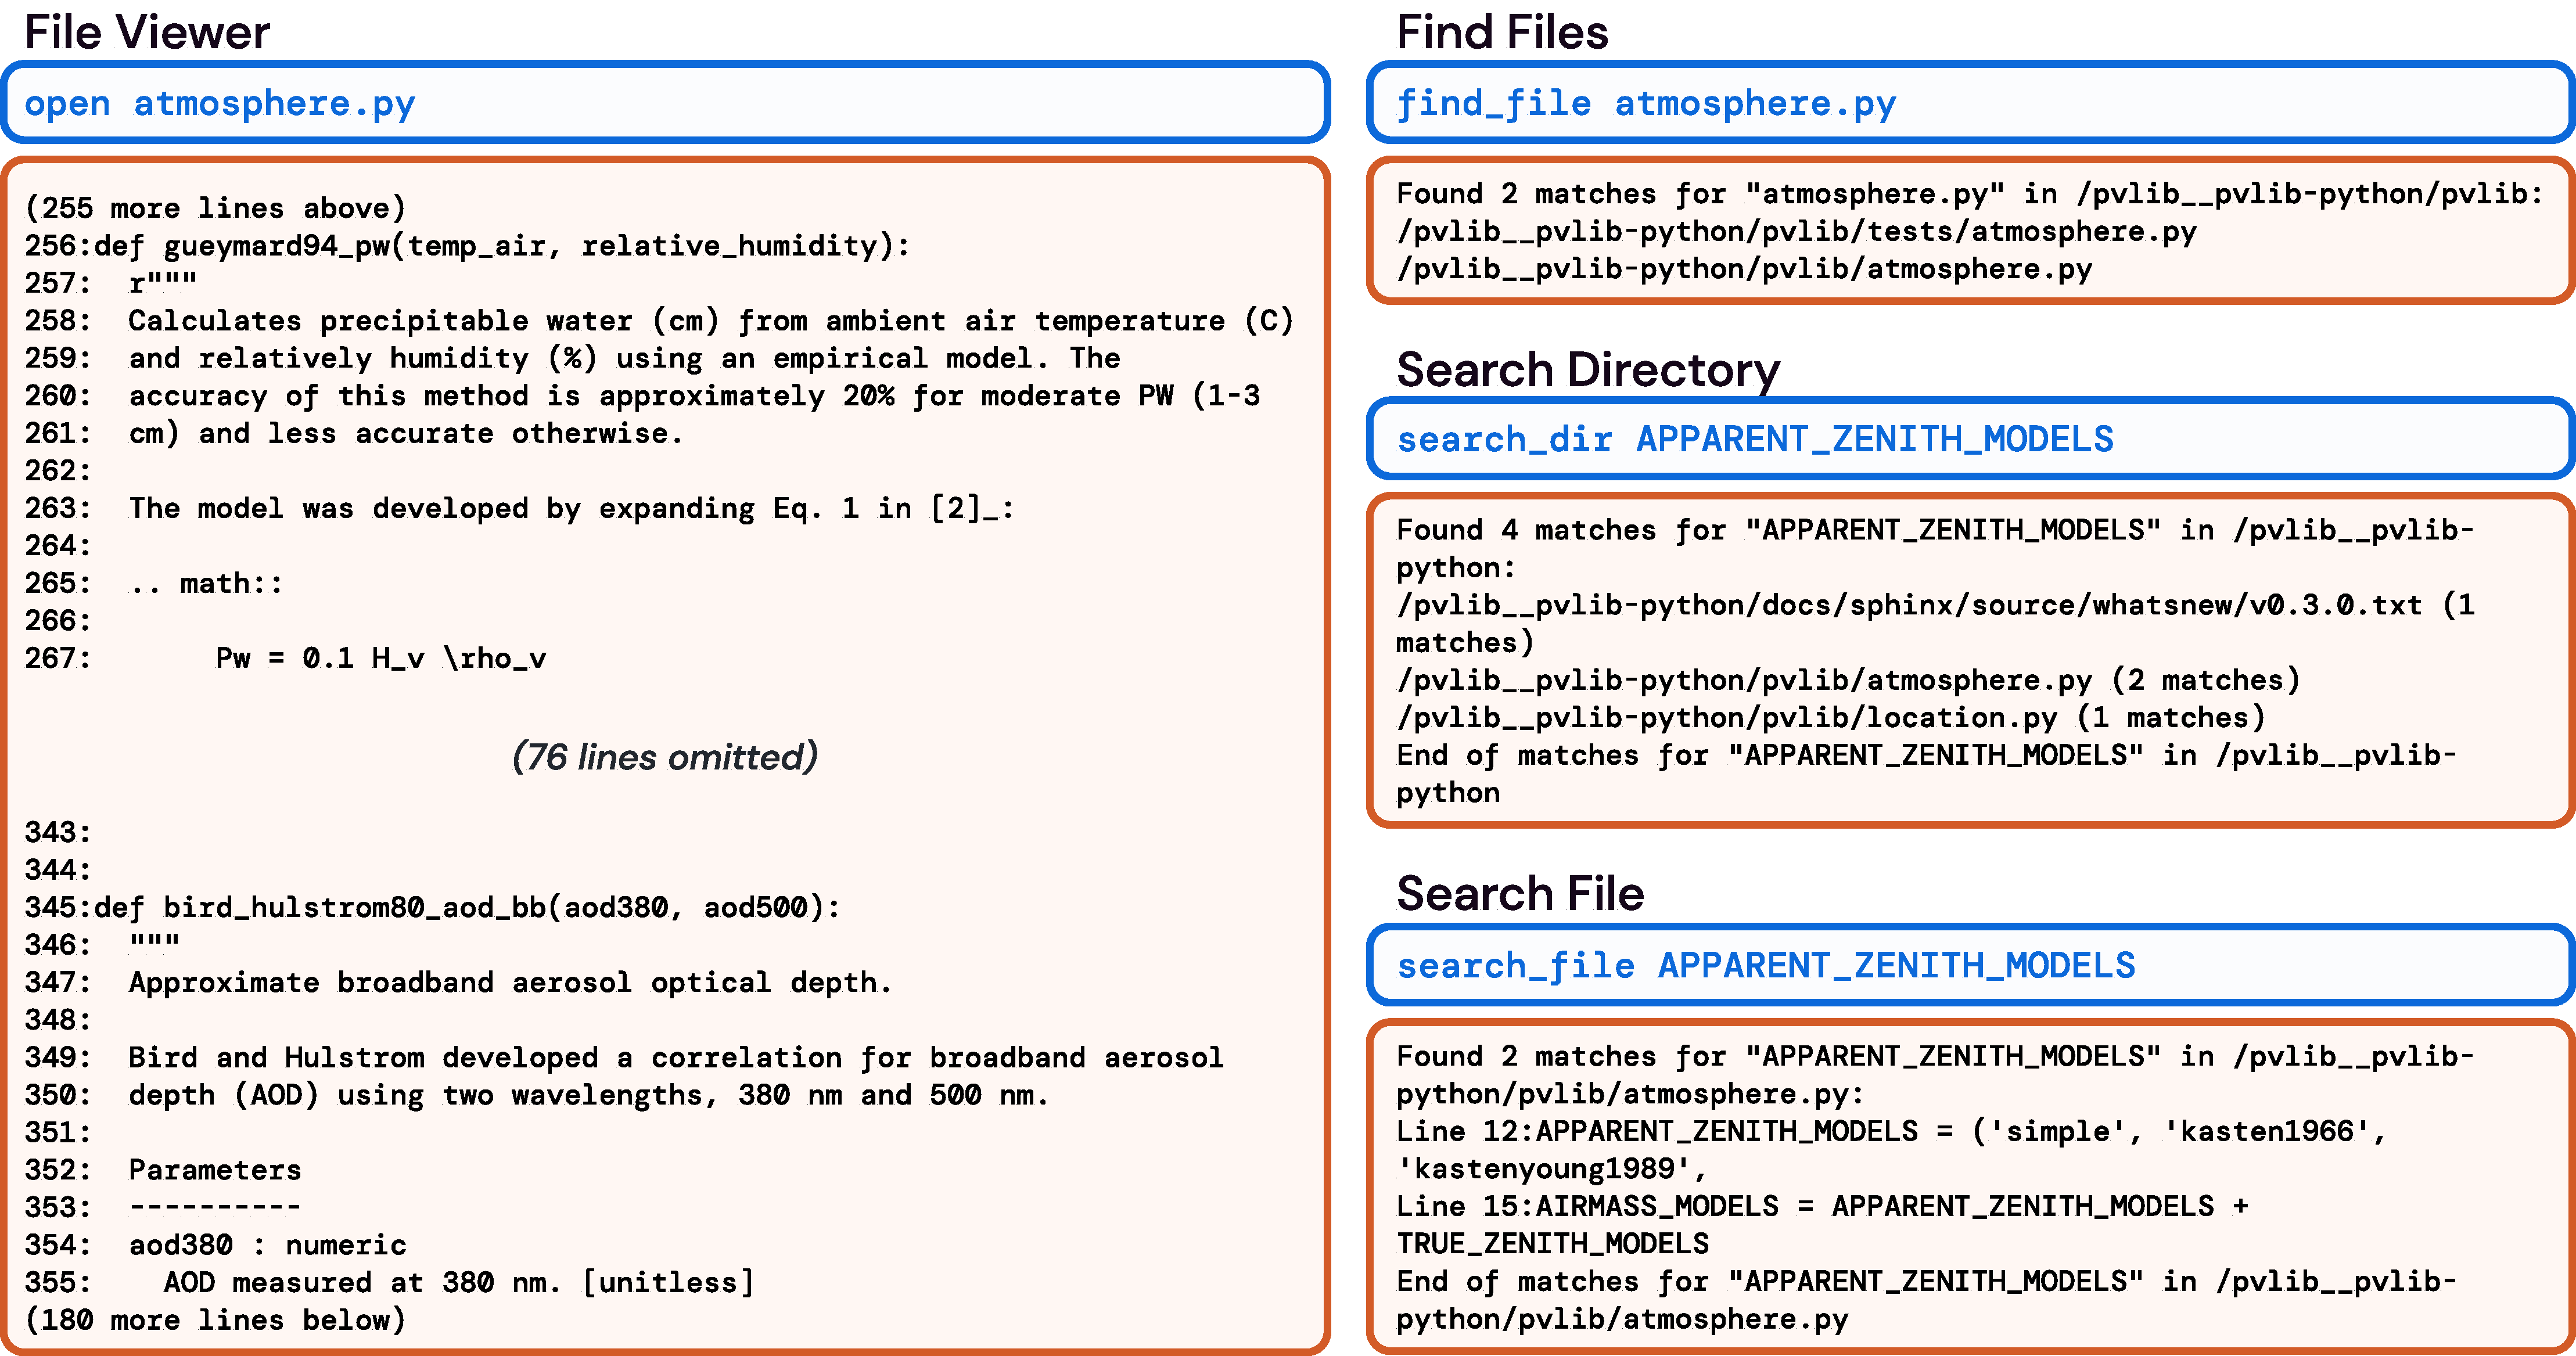
\includegraphics[width=1.0\linewidth]{figures/appx/swe-agent-components.pdf}
    \caption{The File Viewer and Search components of the SWE-agent interface. The corresponding commands for each component are shown in blue. These examples are copied from trajectories generated by SWE-agent w/ GPT-4 Turbo on the \texttt{pvlib\_\_pvlib-python-1603} task instance.}
    \label{fig.appx.swe_agent_components}
\end{figure}

\paragraph{File editor.}
The File Editor, working in conjunction with the File Viewer, primarily refers to the \texttt{edit} command and the guardrails it enforces to protect models against self-incurred cascading edit errors.
Editing and testing are crucial to language agents' success on programming tasks, and a well-designed interface directly influences how well an agent's capabilities can be elicited.
In other words, a bad interface undermines model performance.

As discussed in Section~\ref{sec:sweagent}, editing can be very difficult in a Shell-only setting.
Built in commands (e.g., \texttt{sed}) often require a lengthy list of arguments, and the mis-specification of an argument can easily throw a model off track as it attempts to correct self-incurred errors.
We also observe that when agents use such commands directly, they struggle with the arithmetic skills required to generate an edit.
Details such as including the correct indentation level, inserting delimiters at specific points in a line, and adhering to stylistic preferences of the codebase all require some amount of planning or calculation.
Similar to the Shell-only file viewing process, file editing may also require repeating many commands.
For instance, performing a multi-line edit can only be represented as multiple \texttt{sed} calls with requisite, delicate tweaks to the arguments for every turn.
Furthermore, as referenced in Section~\ref{sec:analysis:interface-design}, editing in Shell-only is usually a ``silent" procedure.
Confirming whether an edit succeeded and viewing its effects requires additional steps that can bloat the editing process with extra, needless commands.

The \texttt{edit} command, documented in Table~\ref{tab:commands}, addresses the Shell-only failure modes by being grounded in the File Viewer standard output.
The line numbers argument eliminates the need for any additional arithmetic, and the find-and-replace edit mechanism is a format that existing models are more used to.
With this functionality, agents can also perform multi-line edits in a single action.

Finally, as mentioned in Section~\ref{sec:analysis:agent-behavior}, an important feature of the \texttt{edit} command is that it does not apply changes which incur a linting error.
A fair and verified assumption we make when considering this feature is that the original codebase associated with each task instance is well-formed.
In other words, we assume that codebase maintainers will only push syntactically sound code that can be compiled successfully.
When an agent issues an edit, it is applied to the codebase.
Then, we run the following linting command (\texttt{CURRENT\_FILE} refers to the file that is currently open):

\texttt{flake8 ---isolated ---select=F821,F822,F{831},E{111},E{112},E{113},E{999},E{902} "\$CURRENT\_FILE" {2}>\&{1}}

The arguments for \texttt{select} are error codes that refer to syntax issues such as indentation.
F\num{821} and F\num{822} indicate undefined names/symbols.
F\num{831} indicates a duplicate argument in a function definition.
E\num{111}, E\num{112}, E\num{113} are indentation errors.
E\num{999} denotes a syntax error and an E\num{902} occurs if flake\num{8} cannot read the source file.

If the edit does not introduce any of these errors, this command will produce no output.
The edit is kept and the updated file content is shown using the File Viewer centered around the lines the edit occurred.
If however the linting command produces output, which indicates the edit introduces a syntax error, the edit is reverted.
In place of the file viewer, a message shown in Figure~\ref{fig.prompts.linting} is displayed to the agent which shows the error that was caused, what the edit would have looked like, and the original file content.
During the development process, we experimented with variations to this message, including the omission of one or more parts.
Our takeaway was that having all three messages is helpful.
Without the error type, the agent might misdiagnose what the mistake was.
Without a snippet of the changed file content, the agent will re-issue the same command more frequently.
Without a snippet of the original file content, the agent has to attend to the same content from several turns ago; agents also sometimes generate \texttt{edit}'s with respect to wrong, errant file content because it is from a more recent turn.

{
\captionsetup{type=figure}
\begin{fileviewerbox}{Linting Error Message}
\begin{Verbatim}[breaklines=true]
Your proposed edit has introduced new syntax error(s). Please understand the fixes and retry your edit commmand.

ERRORS:
- F821 undefined name 'orientation_strategy'
- F821 undefined name 'orientation_strategy'

This is how your edit would have looked if applied
-------------------------------------------------
[File: /pvlib__pvlib-python/pvlib/modelchain.py (1890 lines total)]
(64 more lines above)
65:def basic_chain(times, latitude, longitude,
66:                module_parameters, temperature_model_parameters,
67:                inverter_parameters,
68:                irradiance=None, weather=None,
69:                surface_tilt=None, surface_azimuth=None,
70:                transposition_model='haydavies',
71:                solar_position_method='nrel_numpy',
72:                airmass_model='kastenyoung1989',
73:                altitude=None, pressure=None,
74:                **kwargs):
(1816 more lines below)
-------------------------------------------------

This is the original code before your edit
-------------------------------------------------
[File: /pvlib__pvlib-python/pvlib/modelchain.py (1891 lines total)]
(64 more lines above)
65:def basic_chain(times, latitude, longitude,
66:                module_parameters, temperature_model_parameters,
67:                inverter_parameters,
68:                irradiance=None, weather=None,
69:                surface_tilt=None, surface_azimuth=None,
70:                orientation_strategy=None,
71:                transposition_model='haydavies',
72:                solar_position_method='nrel_numpy',
73:                airmass_model='kastenyoung1989',
74:                altitude=None, pressure=None,
75:                **kwargs):
(1816 more lines below)
-------------------------------------------------
Your changes have NOT been applied. Please fix your edit command and try again.
You either need to 1) Specify the correct start/end line arguments or 2) Correct your edit code.
DO NOT re-run the same failed edit command. Running it again will lead to the same error.
\end{Verbatim}
\end{fileviewerbox}
\captionof{figure}{
A linting error message.
This is emitted if a model generates an \texttt{edit} command that introduces a syntax error into the codebase.
The error message shows the before and after of the proposed edit along with what error messages were thrown.
The problem with this edit is that it omits the \texttt{orientation\_strategy} field in its edit of the \texttt{basic\_chain} method definition.
}
\label{fig.prompts.linting}
}

The editing guardrail has a drawback.
To a certain degree, it forces some edits to be done in a particular order.
For instance, in Figure~\ref{fig.prompts.linting}, if the model's intention was in fact to remove the \texttt{orientation\_strategy} argument, due to the SWE-agent editing guardrails, it would have to remove all references from the function implementation either at the same time in a single action, or before removing it from the method header if split into two separate actions.
For this particular scenario, the latter is necessary because the file snippet is not large enough to show the entirety of the \texttt{basic\_chain} implementation.
This example highlights the trade-offs between the flexibility and guardrails of a command.
Deciding whether to introduce a guardrail depends on how well it reduces common model errors compared to whether such restrictions hamper models' preferred workflows.

\paragraph{Search \& navigation.}
The File Viewer and File Editor together allow agents to make edits, write tests, and perform localization at a file level.
The Search \& navigation module complements these capabilities by giving agents the tools to perform keyword-driven localization at both a directory level and file level.

As discussed, the main struggles with using built in Shell-only search commands such as \texttt{grep} and \texttt{find} are (1) given a general enough term, they are prone to producing too many search results that can consume an inordinate amount of space in the context window, and (2) they are highly configurable, making search result outcomes potentially inconsistent in appearance.
The alternative to these search utilities is to navigate the file system directly with \texttt{cd} and look at what's in each folder with variations of \texttt{ls} and \texttt{cat}; this kind of approach can take a large number of turns without yielding any particularly useful information.

Figure~\ref{fig.appx.swe_agent_components} visualizes the standard output for the three different search commands.
The \texttt{search\_dir} and \texttt{find\_file} helps agents perform directory level searches.
The reason we provide two commands is due to the kinds of keywords that are present in an issue description (e.g., class references, file names).
The \texttt{search\_file} command allows agents to search for terms at a file-level, which is helpful for efficient fine-grained localization.
Taking a step back, the goal of these search commands is to make it easy for the agent to utilize any signal (e.g., line number, stack trace, natural language) about the root cause of an issue that may be present in the issue description or codebase.
Once again, simpler command usage patterns with consistent output formats are easier for agents to use and reduces the chance for mistakes or irrelevant outputs.

The main guardrail in place for all three search commands is curbing the number of search results to \num{50} or fewer.
The downside is that reporting an error forces the model to generate another search query which can be an expensive operation.
This reflects a trade-off between keeping observations concise and making additional calls to the base LM.

\subsection{Implementation}
\label{appx:interface:implementation}

The SWE-agent codebase is generally composed of three modules: the environment, the agent, and the logging mechanism for saving task episodes into trajectories and patch generations.

\textbf{Environment.}
The SWE-agent environment is heavily influenced by the InterCode library~\citep{yang2023intercode}.
For the general pipeline of agent interactions with the environment, our work directly adopts InterCode's interactive coding task formulation.
The environment integrates large parts of the interaction handling logic from the InterCode-Bash environment, which is essentially the Shell-only setting referenced in the paper.
As a part of this adoption, SWE-agent also uses Docker containers to ensure reproducible and safe execution.
Because of this, SWE-agent's infrastructure makes it easy for a user to swap out the Dockerfile (a domain specific language for defining a container) to support other codebases and programming languages beyond the scope of SWE-bench task instances.
One difference is that SWE-agent makes minor adjustments to the underlying communication logic that transfers actions and observations between the Docker container and agent entity.

\textbf{Agent.}
Beyond serving as an agentic wrapper for facilitating multi-turn queries from an LM, the agent module defines the functions that render the ACI (e.g., context management, commands, interface logic, input/output format) and supports inference for closed/open, API-based/local language models.
The main workflow is to define an interface as a class and/or set of commands, which can then be specified via a configuration file, discussed more thoroughly in Section~\ref{appx:interface:configuration}.
The commands for the top performing SWE-agent with GPT 4 configuration are shown in Table~\ref{tab:commands}.

\textbf{Logging.}
For each task episode, the main artifacts produced are the trajectory, which contains a history of the interactions between the agent and environment, and the final patch generation, which can represents a summary of the changes proposed by the agent during the interaction.
The patch generation can be used directly for SWE-bench~\citep{jimenez2024swebench} evaluation.

\subsection{Configuration}
\label{appx:interface:configuration}
The SWE-agent system is instantiated by three components: an LM, a SWE-bench style dataset or GitHub issue, and a configuration file.
The configuration file serves to specify the design of the ACI.
Iteratively refining the configuration file is the main way we achieved better agent performance and carried out different analyses for the main paper.
In this section, we will present a thorough review of what a SWE-agent configuration file looks like.

An agent-computer interface is generally made up of four categories of configurable components:
\begin{enumerate}
    \item Prompt templates: These prompt templates are used to inform the language model of the task setting, show the list of available commands, augment environment responses with the values of state variables, and provide the initial task setting.
    \item Command files: These files contain the source code of bash or Python functions and scripts. Commands are easily modified, added, and removed through manipulating these files' code contents directly. Documentation added in these files can also be injected into prompts to inform the model of the available commands.
    \item Control flow: Methods for parsing model responses and processing history can be specified through these configuration arguments.
    \item Environment variables: Initial values of variables that may interact with commands and the shell can also be specified in the configuration.
\end{enumerate}

In the following Figure~\ref{fig.prompts.example_configuration}, we include an annotated example of the contents of a configuration file.

{
\begin{fileviewerbox}{Configuration (.yaml)}
\begin{Verbatim}[breaklines=true]
# Prompt Templates: Control how observations of environment are shown to agent
system_template: |
  First `system` message shown to agent
instance_template: |-
  Instance prompt, contains task instance-specific content
next_step_template: |-
  Format template of per-turn observation (Contains standard output from agent's action)
next_step_no_output_template: |-
  Format template of observation when there is no standard output from the agent's action
format_error_template: |-
  Format template of error message (Used when agent's action causes an error)
demonstration_template: |
  Format template for showing a demonstration to the agent
demonstrations:
- `trajectories/<username>/<experiment folder>/*.traj` 
- File is a demonstration of how to solve a task. This could an agent generated trajectory.
- You can include 1+ demonstrations

# Environment States: Define features of the SWEEnv environment
env_variables:
# Default variables for SWEEnv at the beginning of each instance
  CURRENT_FILE: 0
  CURRENT_LINE:
  OVERLAP:
  SEARCH_FILES:
  SEARCH_INDEX:
  SEARCH_RESULTS:
  WINDOW_SIZE:
  START_INDEX:
  END_INDEX:
  START_CURSOR:
  END_CUROSR:
  START_CURSORS_MARK:
  END_CURSOR_MARK:
state_command: |
# `state_command` allows you to update state variables to reflect any aspect of the environment (e.g. current working directory)
  name: state
  code: |
    state() { echo '{"pwd": "'$PWD'"}';

# Action Interface: Define how an agent interacts with the SWEEnv environment
command_files:
- path/to/bash_file.sh
- Each file contains a list of commands implemented in bash
- You can include 1+ command files
parse_command: Reference to functionality for defining command documentation
history_processor: Reference to functionality for controlling agent's message history
parse_function: Parser run on agent output
\end{Verbatim}
\end{fileviewerbox}
\captionsetup{type=figure}
\captionof{figure}{
An example of the configuration file that defines the SWE-agent ACI.
A configuration is represented as a single \texttt{.yaml} file, allowing you to
define the commands that agents may use,
write prompts shown to the agent over the course of a single trajectory,
and control the input/output interface that sits between the agent and environment.
}
\label{fig.prompts.example_configuration}
}

The prompt templates are explained in detail in Section~\ref{appx:prompts}.
The environment variables and command files work in tandem; environment variables make the interfaces stateful, and when commands are invoked, the corresponding states are updated to reflect the changes to the environment and interface.
The \texttt{parse\_command}, \texttt{parse\_function}, and \texttt{history\_processor} all reference implementations declared within the agent module.
The \texttt{parse\_command} file describes how command documentation should be presented to the agent.
The \texttt{parse\_function} is what enforces the input/output formats for the agent.
The \texttt{history\_processor} points to the logic for controlling and modifying the message history enforced at each turn throughout a single task episode.

The configuration-based workflow of SWE-agent makes it easy to test new ACIs by incorporating novel commands, input/output formats, context managers, and more into the existing codebase.
In the following subsections, we showcase existing implementations of several of these components and discuss how they can be extended.

\textbf{Commands.}
We describe how to implement your own commands for the SWE-agent ACI.
As shown in the above Figure~\ref{fig.prompts.example_configuration}, commands are declared as a list of one or more file paths in the \texttt{command\_files} argument.
Individual commands must be declared as separate functions in \texttt{.py} or \texttt{.sh} files.
Every command subscribes to the following skeleton code in Figure~\ref{fig.interface.command_skeleton}.

{
\begin{fileviewerbox}{Command Skeleton Code}
\begin{Verbatim}[breaklines=true]
# @yaml
# signature: [command] [argument(s)]
# docstring: [Brief description of what your command does.]
# arguments:
#   [argument 1 name]:
#       type: [type (i.e. integer, string)]
#       description: [Brief description of this argument]
#       required: [true|false]
#   [argument 2 name]:
#       ...
[command]() {
    # Implementation here
}
\end{Verbatim}
\end{fileviewerbox}
\captionsetup{type=figure}
\captionof{figure}{
The skeleton code for defining a command that can be accessed in the SWE-agent ACI.
The function definition includes both the underlying implementation along with several arguments that describe how to use the command, which is compiled into the System template's command documentation at run time.
}
\label{fig.interface.command_skeleton}
}

The choice of Python or Bash based implementations of commands means they can be written to do a wide variety of actions, and the use of Docker means that the commands and system can be co-designed.
Here is a list of guidelines around how to implement commands correctly.
\begin{itemize}[noitemsep]
    \item Command arguments can be referenced via positional parameters notation (i.e. \texttt{\$1}).
    \item If there are no arguments, omit the \texttt{arguments} section.
    \item The implementation for your command is unconstrained. There are no limitations on the form of the underlying command code.
    \item The minimal documentation requirements are \texttt{signature} and \texttt{docstring}.
    \item Global variables can be used to make stateful changes to the environment. For instance, for the commands associated with the File Viewer, you'll see we define the \texttt{CURRENT\_LINE} variable for the file viewer. This variable is modified across multiple commands, including \texttt{open}, \texttt{goto}, \texttt{scroll\_up}, \texttt{scroll\_down}, and \texttt{edit}.
    \item Third party libraries can be freely imported and used by commands (e.g., \texttt{flake8}).
    \item To show effects of a command, print to standard output (e.g., with \texttt{echo}). The command parsing logic is implemented such that it does not look for a return value.
\end{itemize}

Once the file path containing the command is added to \texttt{command\_docs} as an argument, the command is immediately available for use in subsequent task episodes.
Including a demonstration that uses more complicated commands can be helpful to showcase proper use and may increase the frequency with which the agent uses the command.

\textbf{Input/output format.}
The input/output format defines what a correctly formatted response for an agent should look like.
Selecting a suitable format greatly affects how well agents can interact with the environment.
The methods for communicating and enforcing the input/output format are separated across several arguments.
In Figure~\ref{fig.prompts.example_configuration}, the value of \texttt{parse\_function} should point to a class definition that enforces the format and actually parses the agent's responses.
Informing the agent of the expectations around the input/output format should take place in \texttt{system\_template}, and the agent can be reminded of these standards via the \texttt{format\_error\_template}.
New input/output formats can be easily devised and enforced by updating these arguments to point to a new class or display different natural language instructions.

\textbf{Context management.}
Context management is implemented as a class within the agent module.
The \texttt{history\_processor} argument allows one to specify which context manager to use via the configuration file.
Underneath the hood, the context manager is invoked per turn of the interactive loop.
From the entire recorded history of the agent's interactions so far, the context manager constructs the literal history to be fed to the agent to invoke the next response.
The general design of \texttt{history\_processor}s allows for easy experimentation towards more sophisticated strategies for managing history.
